%! TEX root = ../thesis_pres.tex

\section{Approach}
\label{sec:approach}

\subsection{PTAM method}
\label{sub:ptam_method}


\begin{frame}[t]{PTAM method}
  
  \begin{itemize}
    \item PTAM is based on keyframes
    \item The PTAM~\cite{KleinMurray2007} relocalization method has two main steps
      \begin{itemize}
        \item \textbf{Place Finder}: Given a new frame, it finds the closest keyframe
        \item \textbf{Relative Pose Finder}: Once the closest frame is found, its transformation to the new frame is calculated
      \end{itemize}
  \end{itemize}
\end{frame}

\subsection{PTAM Place Finder}
\label{sub:ptam_place_finder}


\begin{frame}[t]{PTAM Place Finder}
  The squared difference between \textit{Small Blurry image} is taken as a measure of distance. Cross Correlation distance.
  \only<1>{

  \begin{columns}
    \begin{column}{0.4\textwidth}
      
      \begin{block}{\textit{Small Blurry image}}
        \begin{itemize}
          \item Size $40 \times 30$
          \item Zero mean
          \item Blurred with Gaussian $\sigma = 2.5$
        \end{itemize}
      \end{block}

    \end{column}
    \begin{column}{0.6\textwidth}
      
      \begin{equation}
        d_{CC} = \sum_{x,y} [(I(x,y) - \bar{I}) - (G(x,y) - \bar{G})]^2
        \label{eq:CC}
      \end{equation}

    \end{column}
  \end{columns}
}

\only<2>{
  \centering
      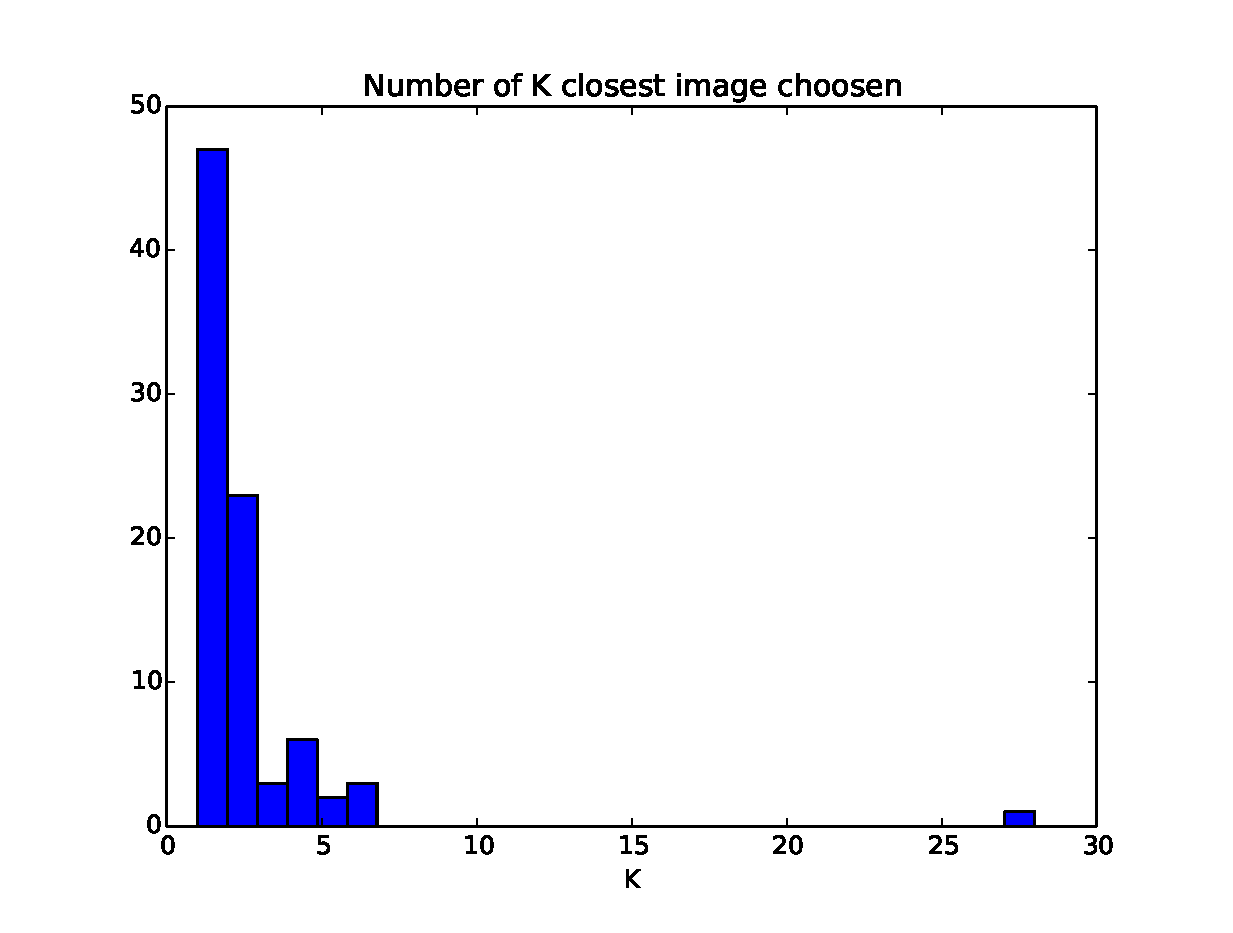
\includegraphics[width=0.7\linewidth]{demo_1_1_CC_choose_distribution.eps}
    }
\end{frame}

\subsection{PTAM Relative Pose Finder}
\label{sub:ptam_relative_pose_finder}



\begin{frame}[t]{PTAM Rrelative Pose Finder}
  \begin{block}{Image Alignment}
    The found keyframe and the new image are aligned over translation and rotation, $SE(2)$. Extended Second-Order Minimization (ESM)~\cite{lovegrove2012parametric} is used.
  
  \end{block}
  
  \only<2>{
  \begin{equation}
    W(x;p) = 
    \begin{bmatrix}
      cos (\alpha) & sin(\alpha) & t_x\\
      -sin(\alpha) & cos(\alpha) & t_y\\
      0 & 0 & 1 \\
    \end{bmatrix}
    \begin{bmatrix} x \\ y \\ 1 \end{bmatrix}
    =
    \begin{bmatrix}
      xcos(\alpha) + y sin(\alpha) + t_x \\
      -x sin(\alpha) + y cos(\alpha) + t_y \\
    \end{bmatrix}
    \label{eq:se2_warp_function}
  \end{equation}
  \begin{equation}
    \min_{p}  \sum_x [I(W(x;p)) - T(x)]^2
    \label{eq:delta_error}
  \end{equation}
  }

  \only<3>{
    \centering
    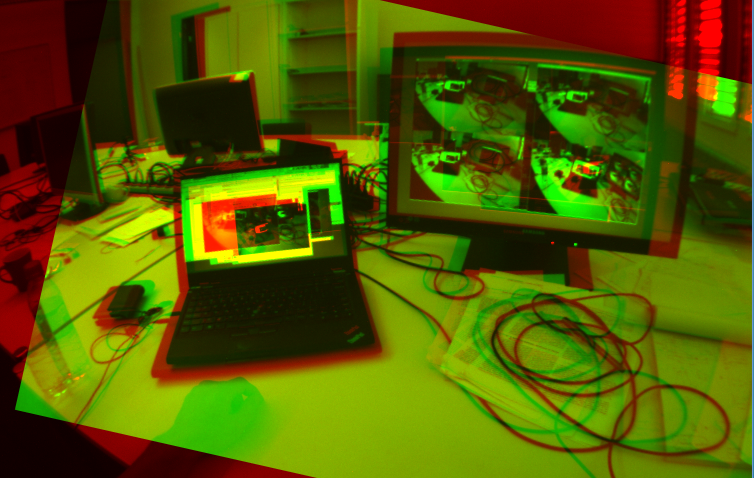
\includegraphics[width=0.7\linewidth]{se2_error_1.png}
  }
\end{frame}

\begin{frame}[t]{3D Interpretations}

  \begin{itemize}
    \item The found transformation can be interpreted in different ways from the world frame.
    \item It is interpreted as world frame rotations, $SO(3)$.
    \item An optimization framework is used to find the best approximations.
  \end{itemize}

  \only<2>{
    \quad
    \begin{equation}
      \delta_i(\xi) = T_{SE(2)}u_i - \pi(T_{SO(3)}(\xi) p_i) \qquad \text{where} \quad u_i = \pi(p_i)
      \label{equ:so3_error}
    \end{equation}
  }

  \only<3>{
    \begin{figure}[htpb]
      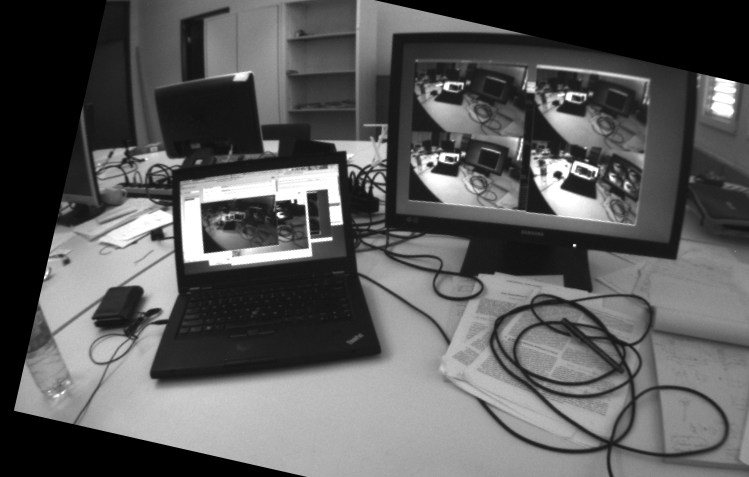
\includegraphics[width=0.45\linewidth]{img/se2_transformation_1.png}
      %\caption{$SE(2)$ transformed image}
      %\label{fig:se2_transformation_1}
      \quad
      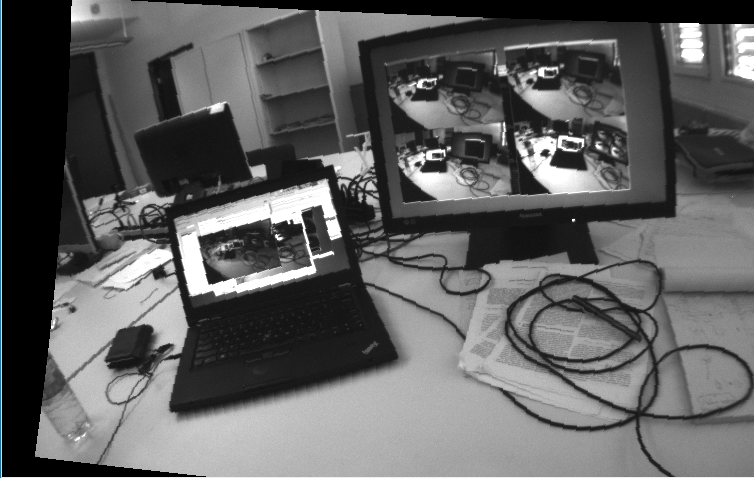
\includegraphics[width=0.45\linewidth]{img/so3_transformation_1.png}
      \caption{$SE(2)$ transformed image. $SO(3)$ transformed image}
      %\label{fig:so3_transformation_1}
    \end{figure}
  }

\end{frame}

\subsection{Geometric Alternative}
\label{sub:geometric_alternative}

\begin{frame}[t]{Geometric Relative Pose Finder}
  \begin{itemize}
    \item Every keyframe has a world frame point associated to every featured point
    \uncover<2->{\item Relate featured points from the new frame to featured points from the keyframe}
    \uncover<3->{\item Use P3P to find the camera pose}
  \end{itemize}

  \only<1>{
    \centering
    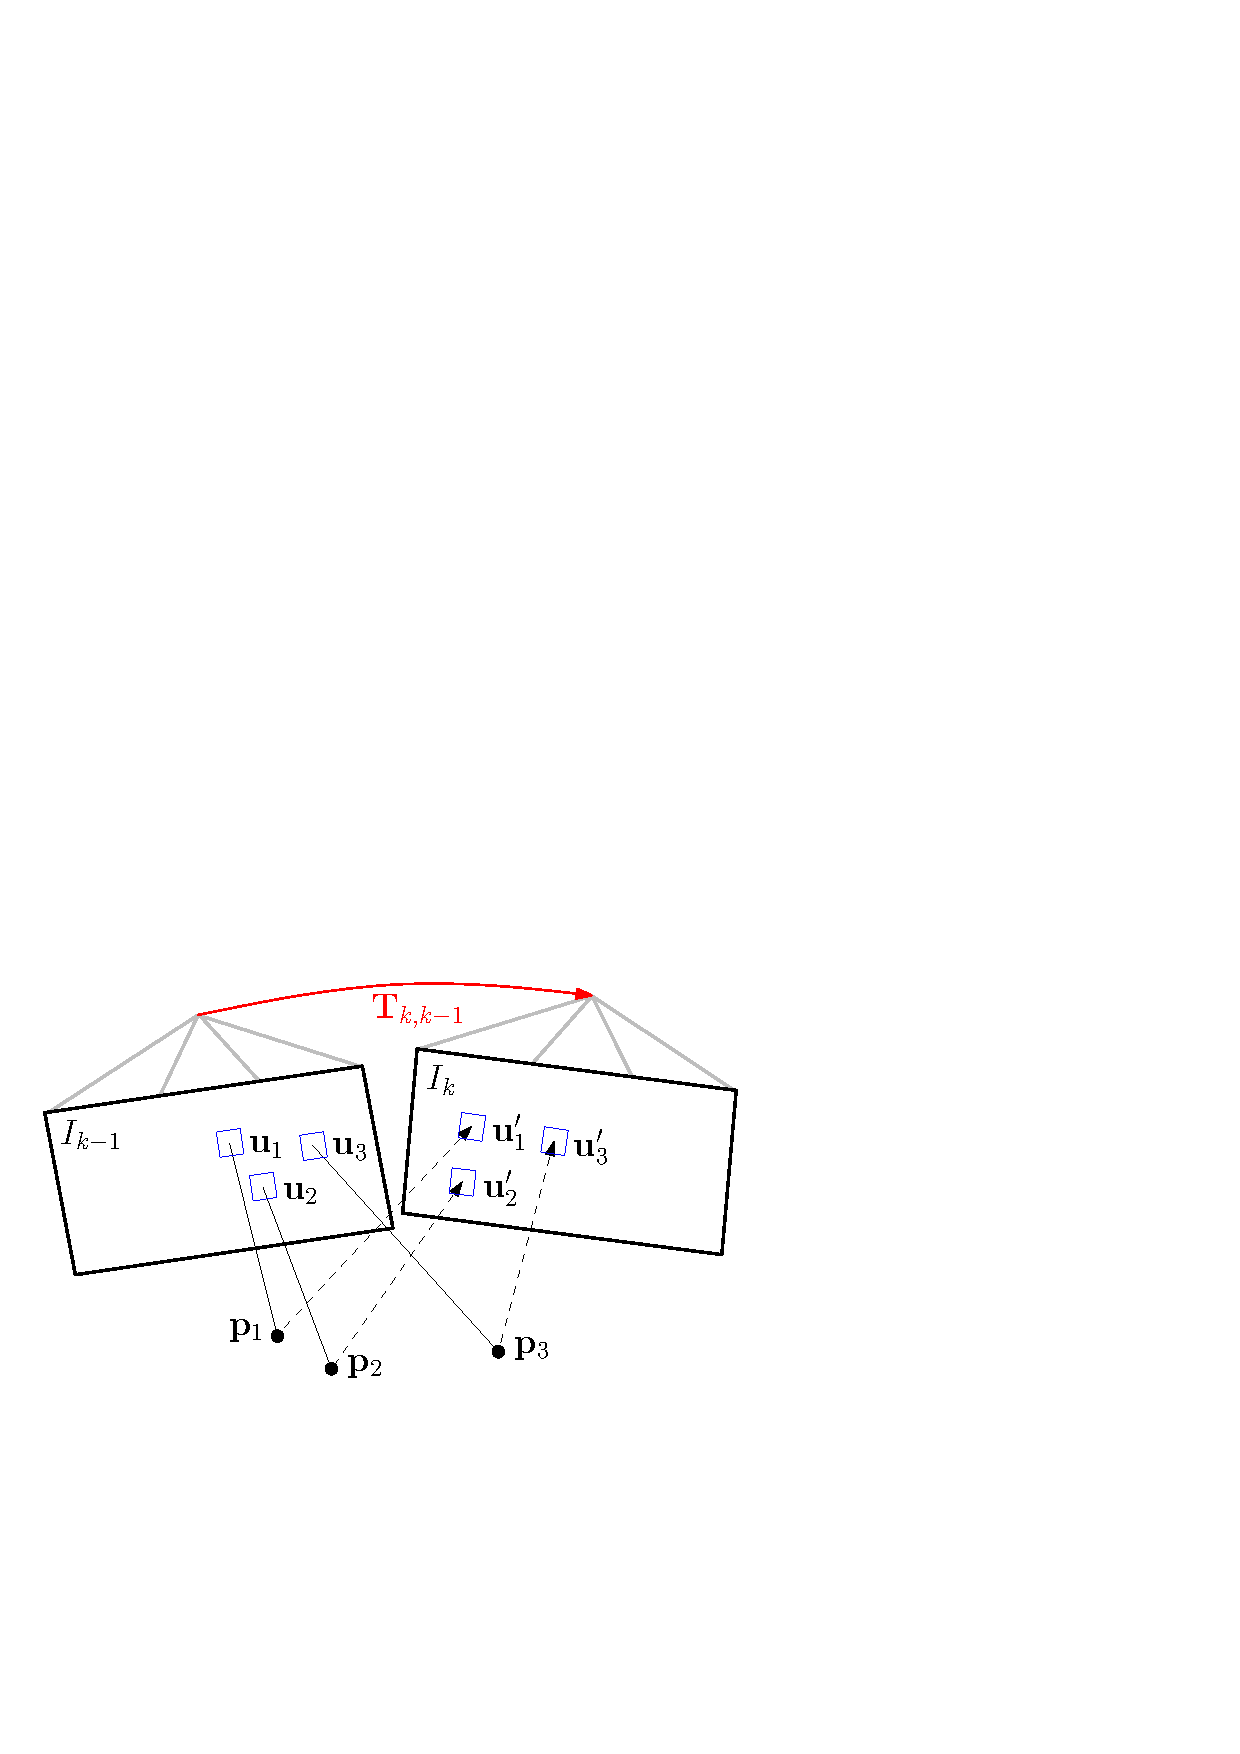
\includegraphics[width=0.6\linewidth]{sparse_img_alignment.pdf}
  }

  \only<2>{
    \centering
    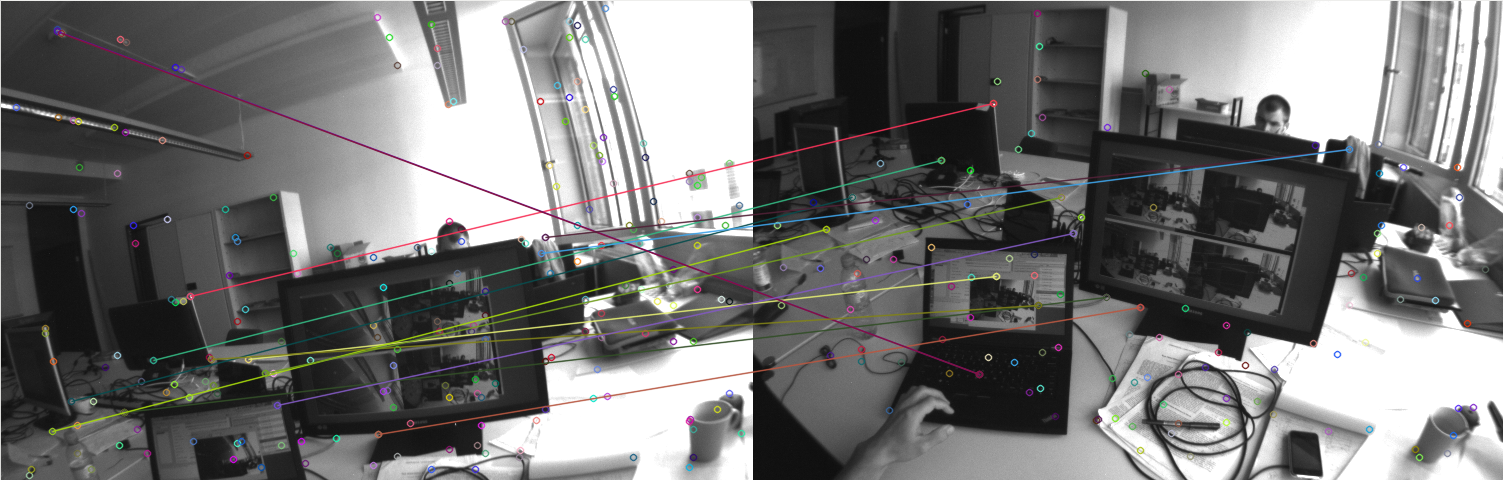
\includegraphics[width=1\linewidth]{3pt_matches_3.png}
  }

  \only<3>{
    \centering
    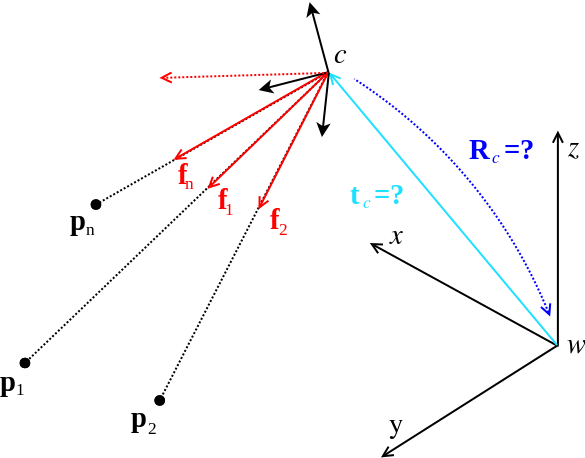
\includegraphics[width=0.5\linewidth]{absolute_central.png}
  }

\end{frame}

\subsection{Ferns Relocalizer}
%\label{sub:ferns_relocalizer}

\begin{frame}[t]{\textit{Ferns} relocalizer}

  \begin{itemize}
    \item Use classifier to model every world frame point with all its views
    \item Every world frame point is a class
    \item Multiple views of the point are used to train
      \begin{itemize}
        \item Artificially generated views are used as well
      \end{itemize}
    \item Finally, P3P is applied to the found points to find the camera transformation
    %\item More than 1700 classes
  \end{itemize}


\end{frame}

\begin{frame}[t]{\textit{Ferns} relocalizer}
  \begin{itemize}
    \item A \textit{fern}~\cite{Ozuysal2010} is a set of randomly generated binary tests on a patch
    \uncover<2->{\item Every \textit{fern} evaluation refers to a class posterior probability distribution}
    \uncover<3->{\item Many \textit{ferns} are used in a classifier}
    %\uncover<3->{\item The set of binary tests can be interpreted as binary and used as an index}
  \end{itemize}

  \centering
  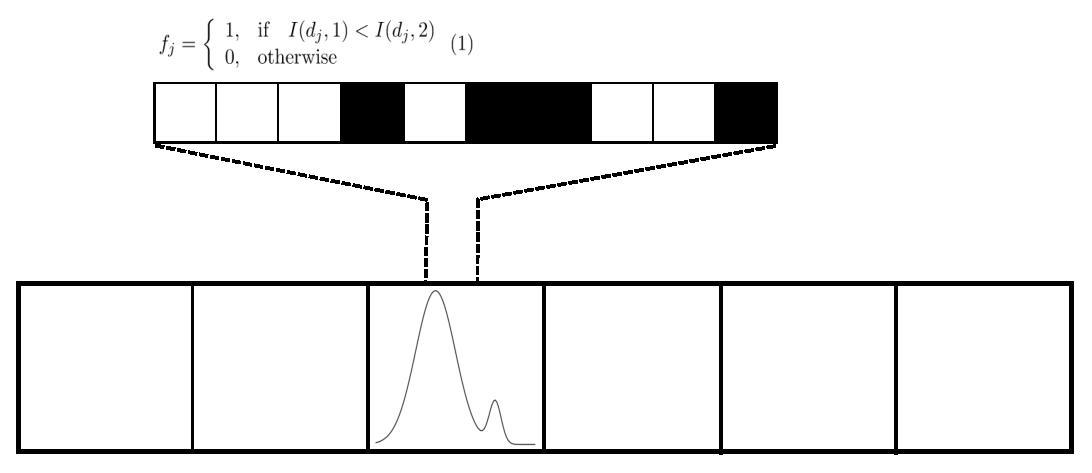
\includegraphics[width=0.9\linewidth]{ferns_figure/ferns_figure.eps}
\end{frame}


